\subsection{Ohm’s Law and Circuit Calculations}
\label{subsec:ohms-law}

Ohm's Law is one of the most fundamental principles in electrical engineering, and it’s as simple as it is powerful. It describes the relationship between voltage (\(E\)), current (\(I\)), and resistance (\(R\)) in a circuit. The law is often summarized by the equation:

\begin{equation}
    E = I \times R
    \label{eq:ohms-law}
\end{equation}

This equation tells us that the voltage across a resistor is equal to the current flowing through it multiplied by its resistance. But wait, there’s more! Ohm’s Law can be rearranged to solve for any of the three variables, depending on what you’re trying to find. For example, if you want to calculate current, you can rearrange the equation to:

\begin{equation}
    I = \frac{E}{R}
    \label{eq:current}
\end{equation}

Similarly, if you need to find resistance, you can use:

\begin{equation}
    R = \frac{E}{I}
    \label{eq:resistance}
\end{equation}

These formulas are your best friends when it comes to analyzing circuits. Let’s break it down further.

\begin{figure}[h]
    \centering
    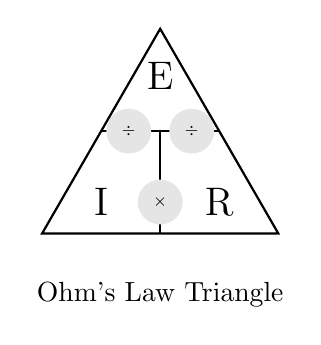
\begin{tikzpicture}
        % Draw the triangle
        \draw[thick] (0,0) -- (3,0) -- (1.5,2.6) -- cycle;
        
        % Add the dividing lines
        \draw[thick] (1.5,0) -- (1.5,1.3);
        \draw[thick] (0.75,1.3) -- (2.25,1.3);
        
        % Add the variables
        \node at (1.5,2.0) {\Large E};  % Voltage at top
        \node at (0.75,0.4) {\Large I}; % Current at bottom left
        \node at (2.25,0.4) {\Large R}; % Resistance at bottom right
        
        % Add multiplication and division symbols in filled circles
        \node[circle, fill=black!10, minimum size=0.02cm] at (1.5,0.4) {\tiny $\times$};  % Multiplication symbol
        \node[circle, fill=black!10, minimum size=0.02cm] at (1.1,1.3) {\tiny $\div$};    % Division symbol
        \node[circle, fill=black!10, minimum size=0.02cm] at (1.9,1.3) {\tiny$\div$};    % Division symbol
        
        % Optional: Add a caption below
        \node[below] at (1.5,-0.5) {Ohm's Law Triangle};
    \end{tikzpicture}
    \caption{Ohm's Law Triangle: To find any value, cover that letter and perform the operation shown between the remaining letters. For voltage (E), multiply I × R. For current (I), divide E ÷ R. For resistance (R), divide E ÷ I.}
    \label{fig:ohms-law-triangle}
\end{figure}

\subsubsection*{Calculating Current}
To calculate current, you need to know the voltage and resistance in the circuit. Using Equation \ref{eq:current}, you can find the current by dividing the voltage by the resistance. For example, if you have a circuit with a 12-volt battery and a 4-ohm resistor, the current would be:

\[
I = \frac{12\,\text{V}}{4\,\Omega} = 3\,\text{A}
\]

\subsubsection*{Calculating Voltage}
If you know the current and resistance, you can calculate the voltage using Equation \ref{eq:ohms-law}. For instance, if a circuit has a current of 2 amperes and a resistance of 5 ohms, the voltage would be:

\[
E = 2\,\text{A} \times 5\,\Omega = 10\,\text{V}
\]

\subsubsection*{Calculating Resistance}
Finally, if you know the voltage and current, you can find the resistance using Equation \ref{eq:resistance}. For example, if a circuit has a voltage of 9 volts and a current of 3 amperes, the resistance would be:

\[
R = \frac{9\,\text{V}}{3\,\text{A}} = 3\,\Omega
\]

\subsubsection*{Series and Parallel Circuits}
In a series circuit, the current is the same through all components, but the voltage across each component can vary. This is because the total resistance in a series circuit is the sum of all individual resistances. On the other hand, in a parallel circuit, the voltage is the same across all components, but the current can vary. The total resistance in a parallel circuit is less than the smallest individual resistance.


\begin{figure}[h!]
    \centering
    \begin{tikzpicture}
        % Series Circuit (left side)
        \draw (0,0) to[battery1] (0,2);
        \draw (0,2) to[R=$R_1$] (2,2);
        \draw (2,2) to[R=$R_2$] (4,2);
        \draw (4,2) to[R=$R_3$] (6,2);
        \draw (6,2) -- (6,0);
        \draw (6,0) -- (0,0);
        \node[below] at (3,-0.5) {Series Circuit};
        
        % Parallel Circuit (right side)
        \begin{scope}[xshift=10cm]
            \draw (0,0) to[battery1] (0,3);
            \draw (0,3) -- (1,3);
            \draw (0,0) -- (1,0);
            \draw (1,3) to[R=$R_1$] (1,0);
            \draw (1,3) -- (3,3);
            \draw (1,0) -- (3,0);
            \draw (3,3) to[R=$R_2$] (3,0);
            \draw (3,3) -- (5,3);
            \draw (3,0) -- (5,0);
            \draw (5,3) to[R=$R_3$] (5,0);
            \node[below] at (3,-0.5) {Parallel Circuit};
        \end{scope}
        
        % Add current flow arrows and voltage labels
        \draw[-latex] (2,1) node[above] {$I$} -- (4,1);
        \draw[-latex] (11.5,2.3) node[above] {$I_1$} -- (11.5,1.9);
        \draw[-latex] (13.5,2.3) node[above] {$I_2$} -- (13.5,1.9);
        \draw[-latex] (15.5,2.3) node[above] {$I_3$} -- (15.5,1.9);
    \end{tikzpicture}
    \caption{Series vs. parallel circuits. In a series circuit (left), the same current flows through all components, while voltage is divided. In a parallel circuit (right), voltage is the same across all components, while current is divided.}
    \label{fig:series-parallel}
\end{figure}


\subsubsection{Questions}

\begin{tcolorbox}[colback=gray!10!white,colframe=black!75!black,title={T5D01}]
    What formula is used to calculate current in a circuit?
    \begin{enumerate}[label=\Alph*),noitemsep]
        \item \(I = E R\)
        \item \textbf{\(I = E / R\)}
        \item \(I = E + R\)
        \item \(I = E - R\)
    \end{enumerate}
\end{tcolorbox}
The correct formula for calculating current is \(I = E / R\), as shown in Equation \ref{eq:current}. The other options are incorrect because they either multiply, add, or subtract the voltage and resistance, which doesn’t make sense in the context of Ohm’s Law.

\begin{tcolorbox}[colback=gray!10!white,colframe=black!75!black,title={T5D02}]
    What formula is used to calculate voltage in a circuit?
    \begin{enumerate}[label=\Alph*),noitemsep]
        \item \textbf{\(E = I \times R\)}
        \item \(E = I / R\)
        \item \(E = I + R\)
        \item \(E = I - R\)
    \end{enumerate}
\end{tcolorbox}
The correct formula for calculating voltage is \(E = I \times R\), as shown in Equation \ref{eq:ohms-law}. The other options are incorrect because they either divide, add, or subtract the current and resistance, which doesn’t align with Ohm’s Law.

\begin{tcolorbox}[colback=gray!10!white,colframe=black!75!black,title={T5D03}]
    What formula is used to calculate resistance in a circuit?
    \begin{enumerate}[label=\Alph*),noitemsep]
        \item \(R = E \times I\)
        \item \textbf{\(R = E / I\)}
        \item \(R = E + I\)
        \item \(R = E - I\)
    \end{enumerate}
\end{tcolorbox}
The correct formula for calculating resistance is \(R = E / I\), as shown in Equation \ref{eq:resistance}. The other options are incorrect because they either multiply, add, or subtract the voltage and current, which doesn’t follow Ohm’s Law.

\begin{tcolorbox}[colback=gray!10!white,colframe=black!75!black,title={T5D04}]
    What is the resistance of a circuit in which a current of 3 amperes flows when connected to 90 volts?
    \begin{enumerate}[label=\Alph*),noitemsep]
        \item 3 ohms
        \item \textbf{30 ohms}
        \item 93 ohms
        \item 270 ohms
    \end{enumerate}
\end{tcolorbox}
Using Equation \ref{eq:resistance}, the resistance is calculated as \(R = \frac{90\,\text{V}}{3\,\text{A}} = 30\,\Omega\). The other options are incorrect because they either misapply the formula or perform incorrect calculations.

\begin{tcolorbox}[colback=gray!10!white,colframe=black!75!black,title={T5D05}]
    What is the resistance of a circuit for which the applied voltage is 12 volts and the current flow is 1.5 amperes?
    \begin{enumerate}[label=\Alph*),noitemsep]
        \item 18 ohms
        \item 0.125 ohms
        \item \textbf{8 ohms}
        \item 13.5 ohms
    \end{enumerate}
\end{tcolorbox}
Using Equation \ref{eq:resistance}, the resistance is calculated as \(R = \frac{12\,\text{V}}{1.5\,\text{A}} = 8\,\Omega\). The other options are incorrect because they either misapply the formula or perform incorrect calculations.

\begin{tcolorbox}[colback=gray!10!white,colframe=black!75!black,title={T5D06}]
    What is the resistance of a circuit that draws 4 amperes from a 12-volt source?
    \begin{enumerate}[label=\Alph*),noitemsep]
        \item \textbf{3 ohms}
        \item 16 ohms
        \item 48 ohms
        \item 8 ohms
    \end{enumerate}
\end{tcolorbox}
Using Equation \ref{eq:resistance}, the resistance is calculated as \(R = \frac{12\,\text{V}}{4\,\text{A}} = 3\,\Omega\). The other options are incorrect because they either misapply the formula or perform incorrect calculations.

\begin{tcolorbox}[colback=gray!10!white,colframe=black!75!black,title={T5D07}]
    What is the current in a circuit with an applied voltage of 120 volts and a resistance of 80 ohms?
    \begin{enumerate}[label=\Alph*),noitemsep]
        \item 9600 amperes
        \item 200 amperes
        \item 0.667 amperes
        \item \textbf{1.5 amperes}
    \end{enumerate}
\end{tcolorbox}
Using Equation \ref{eq:current}, the current is calculated as \(I = \frac{120\,\text{V}}{80\,\Omega} = 1.5\,\text{A}\). The other options are incorrect because they either misapply the formula or perform incorrect calculations.

\begin{tcolorbox}[colback=gray!10!white,colframe=black!75!black,title={T5D08}]
    What is the current through a 100-ohm resistor connected across 200 volts?
    \begin{enumerate}[label=\Alph*),noitemsep]
        \item 20,000 amperes
        \item 0.5 amperes
        \item \textbf{2 amperes}
        \item 100 amperes
    \end{enumerate}
\end{tcolorbox}
Using Equation \ref{eq:current}, the current is calculated as \(I = \frac{200\,\text{V}}{100\,\Omega} = 2\,\text{A}\). The other options are incorrect because they either misapply the formula or perform incorrect calculations.

\begin{tcolorbox}[colback=gray!10!white,colframe=black!75!black,title={T5D09}]
    What is the current through a 24-ohm resistor connected across 240 volts?
    \begin{enumerate}[label=\Alph*),noitemsep]
        \item 24,000 amperes
        \item 0.1 amperes
        \item \textbf{10 amperes}
        \item 216 amperes
    \end{enumerate}
\end{tcolorbox}
Using Equation \ref{eq:current}, the current is calculated as \(I = \frac{240\,\text{V}}{24\,\Omega} = 10\,\text{A}\). The other options are incorrect because they either misapply the formula or perform incorrect calculations.

\begin{tcolorbox}[colback=gray!10!white,colframe=black!75!black,title={T5D10}]
    What is the voltage across a 2-ohm resistor if a current of 0.5 amperes flows through it?
    \begin{enumerate}[label=\Alph*),noitemsep]
        \item \textbf{1 volt}
        \item 0.25 volts
        \item 2.5 volts
        \item 1.5 volts
    \end{enumerate}
\end{tcolorbox}
Using Equation \ref{eq:ohms-law}, the voltage is calculated as \(E = 0.5\,\text{A} \times 2\,\Omega = 1\,\text{V}\). The other options are incorrect because they either misapply the formula or perform incorrect calculations.

\begin{tcolorbox}[colback=gray!10!white,colframe=black!75!black,title={T5D11}]
    What is the voltage across a 10-ohm resistor if a current of 1 ampere flows through it?
    \begin{enumerate}[label=\Alph*),noitemsep]
        \item 1 volt
        \item \textbf{10 volts}
        \item 11 volts
        \item 9 volts
    \end{enumerate}
\end{tcolorbox}
Using Equation \ref{eq:ohms-law}, the voltage is calculated as \(E = 1\,\text{A} \times 10\,\Omega = 10\,\text{V}\). The other options are incorrect because they either misapply the formula or perform incorrect calculations.

\begin{tcolorbox}[colback=gray!10!white,colframe=black!75!black,title={T5D12}]
    What is the voltage across a 10-ohm resistor if a current of 2 amperes flows through it?
    \begin{enumerate}[label=\Alph*),noitemsep]
        \item 8 volts
        \item 0.2 volts
        \item 12 volts
        \item \textbf{20 volts}
    \end{enumerate}
\end{tcolorbox}
Using Equation \ref{eq:ohms-law}, the voltage is calculated as \(E = 2\,\text{A} \times 10\,\Omega = 20\,\text{V}\). The other options are incorrect because they either misapply the formula or perform incorrect calculations.

\begin{tcolorbox}[colback=gray!10!white,colframe=black!75!black,title={T5D13}]
    In which type of circuit is DC current the same through all components?
    \begin{enumerate}[label=\Alph*),noitemsep]
        \item \textbf{Series}
        \item Parallel
        \item Resonant
        \item Branch
    \end{enumerate}
\end{tcolorbox}
In a series circuit, the current is the same through all components. This is because there’s only one path for the current to flow. In parallel circuits, the current can vary across different branches.

\begin{tcolorbox}[colback=gray!10!white,colframe=black!75!black,title={T5D14}]
    In which type of circuit is voltage the same across all components?
    \begin{enumerate}[label=\Alph*),noitemsep]
        \item Series
        \item \textbf{Parallel}
        \item Resonant
        \item Branch
    \end{enumerate}
\end{tcolorbox}
In a parallel circuit, the voltage is the same across all components. This is because each component is connected directly to the voltage source. In series circuits, the voltage can vary across different components.
